% !TeX encoding = UTF-8
% !TeX spellcheck = pl_PL


% $Id:$

%Author: Wojciech Domski
%Szablon do ząłożeń projektowych, raportu i dokumentacji z steorwników robotów
%Wersja v.1.0.0
%

%% Konfiguracja:
\newcommand{\kurs}{Sterowniki robot\'{o}w}
\newcommand{\formakursu}{Projekt}

%odkomentuj właściwy typ projektu
\newcommand{\doctype}{Za\l{}o\.{z}enia projektowe}
%\newcommand{\doctype}{Raport}
%\newcommand{\doctype}{Dokumentacja}

%wpisz nazwę projektu
\newcommand{\projectname}{Sterowany Pochyleniem R\k{e}ki Pojazd Prawie Autonomiczny}

%wpisz akronim projektu
\newcommand{\acronim}{S.P.R.P.P.A}

%zmaiast X wpisz numer grupy projektowej
\newcommand{\nrgrupy}{6}
%wpisz Imię i nazwisko oraz numer albumu
\newcommand{\osobaA}{Patrycjusz \textsc{Augu\.{s}cik}, 226523}
%w przypadku projektu jednoosobowego usuń zawartość nowej komendy
\newcommand{\osobaB}{Maciej \textsc{Kajdak}, 226256}

%wpisz termin w formie, jak poniżej dzień, parzystość, godzina
\newcommand{\termin}{wtTP11}

%wpisz imię i nazwisko prowadzącego
\newcommand{\prowadzacy}{mgr in\.{z}. Wojciech \textsc{Domski}}

\documentclass[10pt, a4paper]{article}
% W nawiasie klamrowym podana jest klasa dokumentu. Standardowe klasy artykułu
% to: article, amsart, scrartcl, artikel1, artikel2, artikel3.
% W nawiasie prostokątnym deklarowane są opcje dokumentu. Zamiast 10pt
% można podać 11pt lub 12pt. Dokument w dwóch kolumnach uzyskuje się po
% wpisaniu opcji twocolumn, 

\usepackage[MeX]{polski}
\usepackage[utf8]{inputenc}
\usepackage{caption}
\usepackage{float}
\usepackage{lscape}

%Preambuła dokumentu

% linki w spisie tresci, bibliografi
\usepackage[bookmarks=true,bookmarksnumbered=false,unicode=true,pdftex=true, colorlinks,filecolor=black,linkcolor=black,urlcolor=black,citecolor=black]{hyperref}

%ustawienie rozmiaru papieru
\usepackage[a4paper, left=2.5cm, right=2.5cm, top=2.5cm, bottom=2.5cm, headsep=1.2cm]{geometry}

%rozmaite ustawienia pozwalające okreslić język

%NALEŻY wybrać jeden z pakietów
%\usepackage{polski} %przydatne podczas składania dokumentów w j. polskim
\usepackage[polish]{babel}  % pakiet lokalizujący dokument w języku polskim
%\usepackage[british]{babel}

\usepackage{indentfirst}	% polski styl pisania (np. rozpoczecie pierwszego akapitu
% pod nazwa rozdzialu od wciecia)
%\usepackage[OT4]{fontenc}
\usepackage[utf8]{inputenc} % w miejsce utf8 można wpisać latin2 bądź cp1250,
% w zależności od tego w jaki sposób kodowane są 
% polskie znaki diakrytyczne przy wprowadzaniu 
% z klawiatury.
%kodowanie znaków, zależne od systemu
\usepackage[T1]{fontenc} %poprawne składanie polskich czcionek

%OPEROWANIE NA OBRAZACH
\usepackage{graphicx}       % pakiet graficzny, umożliwiający m.in.
% import grafik w formacie eps
%\usepackage{epstopdf}		% pozwala na importowanie grafik w formacie eps
% przy użyciu pdflatex
\usepackage[update,prepend]{epstopdf}
\usepackage{rotating}       % pakiet umożliwiający obracanie rysunków
\usepackage{subfigure}      % pakiet umożliwiający tworzenie podrysunków
\usepackage{epic}           % pakiet umożliwiający rysowanie w środowisku latex
\usepackage{psfrag}         % pakiet umożliwiający podmianę łańcuchów znaków 
% w plikach eps
%\usepackage{curves}         % pakiet do wykreslania krzywych

%pakiety dodające dużo dodatkowych poleceń matematycznych
\usepackage{amsfonts}       % pakiet z rozmaitymi czcionkami matematycznymi
%\usepackage{amssymb}        % pakiet z rozmaitymi symbolami matematycznymi
\usepackage{amsmath}        % pakiet z rozmaitymi środowiskami matematycznymi

\usepackage{fp}             % pakiet z funkcjami operujacymi 
% na liczbach zmiennoprzecinkowych
\usepackage{calc}           % pakiet umożliwiający operacje arytmetyczne
% na tzw. licznikach (liczbach całkowitych)
\usepackage{leftidx}		% indeksy górne i dolne po lewej stronie

%definicje matematyczne
\providecommand{\abs}[1]{\lvert#1\rvert}
\providecommand{\norm}[1]{\lVert#1\rVert}

%pakiety wspomagające i poprawiające składanie tabel
\usepackage{supertabular}
\usepackage{array}
\usepackage{tabularx}
\usepackage{hhline}
\usepackage{longtable}		% wsparcie dla dlugich tabel
\usepackage{multicol}		% podzial strony na wiele kolumn

%pakiet do BibTex
\usepackage{cite}

\usepackage{url} %pakiet pozawalający na dodawanie adresów url w bibliografi

%pakiet wypisujący na marginesie etykiety równań i rysunków zdefiniowanych przez \label{}, chcąc wygenerować finalną wersję dokumentu wystarczy usunąć poniższą linię
%\usepackage{showlabels}

\usepackage{float}			% lepsza obsluga mechanizmow obiektow plywajacych
% wymuszenie wstawienia np. tabeli, obrazka w danym miejscu przez [H]

\usepackage{listings}       % pakiet dedykowany zrodlom programow
\usepackage{color}


\definecolor{dkgreen}{rgb}{0,0.6,0}
\definecolor{gray}{rgb}{0.5,0.5,0.5}
\definecolor{mauve}{rgb}{0.58,0,0.82}

\lstset{ %
	language=Matlab,                % the language of the code
	basicstyle=\scriptsize,           % the size of the fonts that are used for the code
	numbers=left,                   % where to put the line-numbers
	numberstyle=\tiny\color{gray},  % the style that is used for the line-numbers
	stepnumber=1,                   % the step between two line-numbers. If it's 1, each line 
	% will be numbered
	numbersep=5pt,                  % how far the line-numbers are from the code
	backgroundcolor=\color{white},      % choose the background color. You must add \usepackage{color}
	showspaces=false,               % show spaces adding particular underscores
	showstringspaces=false,         % underline spaces within strings
	showtabs=false,                 % show tabs within strings adding particular underscores
	%frame=single,                   % adds a frame around the code
	rulecolor=\color{black},        % if not set, the frame-color may be changed on line-breaks within not-black text (e.g. comments (green here))
	tabsize=2,                      % sets default tabsize to 2 spaces
	captionpos=b,                   % sets the caption-position to bottom
	breaklines=true,                % sets automatic line breaking
	breakatwhitespace=false,        % sets if automatic breaks should only happen at whitespace
	%title=\lstname,                   % show the filename of files included with \lstinputlisting;
	% also try caption instead of title
	keywordstyle=\color{blue},          % keyword style
	commentstyle=\color{dkgreen},       % comment style
	stringstyle=\color{mauve},         % string literal style
	escapeinside={\%*}{*)},            % if you want to add LaTeX within your code
	morekeywords={*,...},              % if you want to add more keywords to the set
	deletekeywords={...}              % if you want to delete keywords from the given language
}

%polish signs in lst code
\lstset{literate=%
	{ą}{{\k{a}}}1
	{ć}{{\'c}}1
	{ę}{{\k{e}}}1
	{ł}{{\l}}1
	{ń}{{\'n}}1
	{ó}{{\'o}}1
	{ś}{{\'s}}1
	{ż}{{\.z}}1
	{ź}{{\'z}}1
	{Ą}{{\k{A}}}1
	{Ć}{{\'C}}1
	{Ę}{{\k{E}}}1
	{Ł}{{\L}}1
	{Ń}{{\'N}}1
	{Ó}{{\'O}}1
	{Ś}{{\'S}}1
	{Ż}{{\.Z}}1
	{Ź}{{\'Z}}1
}

\usepackage{verbatim}       % pakiet dedykowany rozmaitym wydrukom tekstowym
\usepackage{ifthen}         % pakiet umożliwiający tworzenie prostych programów
% (m.in. zawiera instrukcje powtórzeniowe 
% i warunkowe)
\usepackage{upquote}		%normal quotations marks ' and `

% deklaracje wymagane przez pakiet theorem automatycznie ladowany w przypadku
% klasy dokumentu article
%
\newtheorem{Dn}{Definicja}[section]     % deklaracja srodowiska definicja
\newtheorem{La}[Dn]{Lemat}                % deklaracja srodowiska lemat
\newtheorem{Tm}[Dn]{Twierdzenie}          % deklaracja srodowiska twierdzenie
\newtheorem{Rk}[Dn]{Spostrze{\.z}enie}  % deklaracja srodowiska spostrzezenie
\newtheorem{Am}[Dn]{Algorytm}           % deklaracja srodowiska algorytm
\newtheorem{As}[Dn]{Za{\l}o{\.z}enie}   % deklaracja srodowiska zalozenie
\newtheorem{Pn}[Dn]{Propozycja}           % deklaracja srodowiska propozycja
\newtheorem{Py}[Dn]{W{\l}asno{\'s}{\'c}}  % deklaracja srodowiska wlasnosc
\newtheorem{Cy}[Dn]{Wniosek}              % deklaracja srodowiska wniosek
\newtheorem{Ee}[Dn]{Przyk{\l}ad}        % deklaracja srodowiska przyklad
\newtheorem{Ex}{{\'C}wiczenie}          % deklaracja srodowiska cwiczenie

%helps to specify width of a column in table
%\begin{tabular}{|C{1cm}|c|c|c|c|c|c|c|c|c|c|}
%first column will have widht of 1cm
\newcolumntype{L}[1]{>{\raggedright\let\newline\\\arraybackslash\hspace{0pt}}m{#1}}
\newcolumntype{C}[1]{>{\centering\let\newline\\\arraybackslash\hspace{0pt}}m{#1}}
\newcolumntype{R}[1]{>{\raggedleft\let\newline\\\arraybackslash\hspace{0pt}}m{#1}}

\sloppy			%zawija bardzo długie linie

%\pagenumbering{gobble}% Remove page numbers (and reset to 1)
	
\begin{document}

\def\tablename{Tabela}	%zmienienie nazwy tabel z Tablica na Tabela

\begin{titlepage}
	\begin{center}
		\textsc{\LARGE \formakursu}\\[1cm]		
		\textsc{\Large \kurs}\\[0.5cm]		
		\rule{\textwidth}{0.08cm}\\[0.4cm]
		{\huge \bfseries \doctype}\\[1cm]
		{\huge \bfseries \projectname}\\[0.5cm]
		{\huge \bfseries \acronim}\\[0.4cm]
		\rule{\textwidth}{0.08cm}\\[1cm]
		
		\begin{flushright} \large
		\emph{Skład grupy (\nrgrupy):}\\
		\osobaA\\
		\osobaB\\[0.4cm]
		
		\emph{Termin: }\termin\\[0.4cm]

		\emph{Prowadzący:} \\
		\prowadzacy \\
		
		\end{flushright}
		
		\vfill
		
		{\large \today}
	\end{center}	
\end{titlepage}

\newpage
\tableofcontents
\newpage

	\section{Opis projektu i założenia projektowe}
\subsection{Projekt nadajnika wykorzystującego akcelerometr do sterowania pojazdem kołowym}
Projekt zakłada wykorzystanie akcelerometra dostępnego na płytce rozwojowej STM32L476 Discovery do sterowania pojazdem kołowym. Jest to moduł MEMS LSM303CTR z wbudowanym akcelerometrem i magnetometrem. Mikrokontroler będzie łączył się z modułem za pomocą szeregowego  interfejsu urządzeń peryferyjnych -- SPI w trybie Master Receives Only. Komunikacja między samochodzikiem a płytką odbywać się będzie za pomocą układu WiFi + Bluetooth BLE ESP-WROOM-32 - SMD. Z modułem mikrokontroler będzie się łączył dzięki komunikacji UART. W naszym projekcie zostanie wykorzystany tylko moduł bluetooth. Moduł ten w tej części projektu będzie pełnił rolę nadajnika. Pojazd będzie się poruszał w kierunku wskazanym przez dłoń sterującego. Aby połączyć się z samochodzikiem, należy trzymać w dłoni płytkę uruchomieniową, która będzie się łączyć z samochodzikiem automatycznie. 
Możliwości ruchu pojazdu:
\\* -- do przodu
\\* -- do tyłu
\\* -- w lewo
\\* -- w prawo
\\* Prędkość samochodzika będzie uzależniona od szybkości ruchów ręki.


\subsection{Projekt odbiornika i pojazdu kołowego}
Projekt zakłada wykorzystanie układu WiFi + Bluetooth BLE ESP-WROOM-32 - SMD. Z tego modułu zostanie wykorzystany tylko moduł bluetooth jako odbiornik informacji z nadajnika. Do zbudowania pojazdu zostanie wykorzystany stary samochodzik - zabawka. W celu ulepszenia samochodu - zamontujemy nowe silniczki komutatorowe prądu stałego. Pojazd ten będzie mógł osiągnąć dużą prędkość dzięki przekładni 2:1. Wmontujemy również czujniki odległości, a zadaniem pojazdu będzie natychmiastowe zatrzymanie się w przypadku napotkania przeszkody lub w momencie utraty połączenia bluetooth z nadajnikiem.
W opisywanym samochodziku wykorzystamy napęd na przednią oś, silniki zostaną połączone z mostkami H, a całością będzie sterować mikrokontroler.

\subsection{Funkcjonalności dodatkowe}
Nieobowiązkowo projekt zakłada dodanie funkcjonalności zmiany źródła sterowania. Przełączenie sterowania ma się opierać o dodatkową płytkę Raspberry Pi, dzięki której możliwe będzie przetwarzanie obrazu z kamery zamontowanej na samochodziku. Tym sposobem samochodzik miałby się poruszać za określonym przedmiotem (np. małą piłką w mocno jaskrawym kolorze). Przełączenie sterowania miałoby nastąpić po jawnym wybraniu odpowiedniej opcji na płytce Discovery, a do tego celu pomocne będzie użycie wyświetlacza LCD. 




%
%\begin{lstlisting}[tabsize=2]
%int foo(void){
%	return 2;
%}
%\end{lstlisting}
%
%\begin{table}[H]
%	\centering
%	\begin{tabular}{|l|l|}
%		\hline
%		Kolumna A	&	Kolumna B\\
%		\hline
%		1 A			&	1B\\
%		2 A			&	2B\\
%		3 A			&	3B\\
%		4 A			&	4B\\
%		\hline
%	\end{tabular}
%	\caption{Rzędy i kolumny}
%	\label{tab:Tabelka}
%\end{table}
%
%\begin{figure}[H]
%	\centering
%	%poniższą linię odkomentuj oraz podaj ściezkę do obrazka
%	%\includegraphics[width=0.8\textwidth]{grafika/rysunek.png}
%	\caption{Rysunek2}
%	\label{fig:Rysunek2}
%\end{figure}
%
%Przykładowy wzór (\ref{eq:Wzor}):
%\begin{equation}
%\label{eq:Wzor}
%\Theta = \int_t^{t+dt} \omega \, dt.	
%\end{equation}
%
%Cytowanie pracy \cite{Wd14}.

\newpage
\section{Organizacja pracy}
\subsection{Harmonogram zadań}
Harmonogram pracy zespołu wraz z datami terminu został przedstawiony na rysunku \ref{fig:Harmonogram}. Na podstawie danych z harmonogramu rozpoczęto pracę nad rozdziałem pomniejszych zadań. Harmonogram został wygenerowany przy pomocy programu Ganttproject.

\begin{figure}[H]
	\centering
	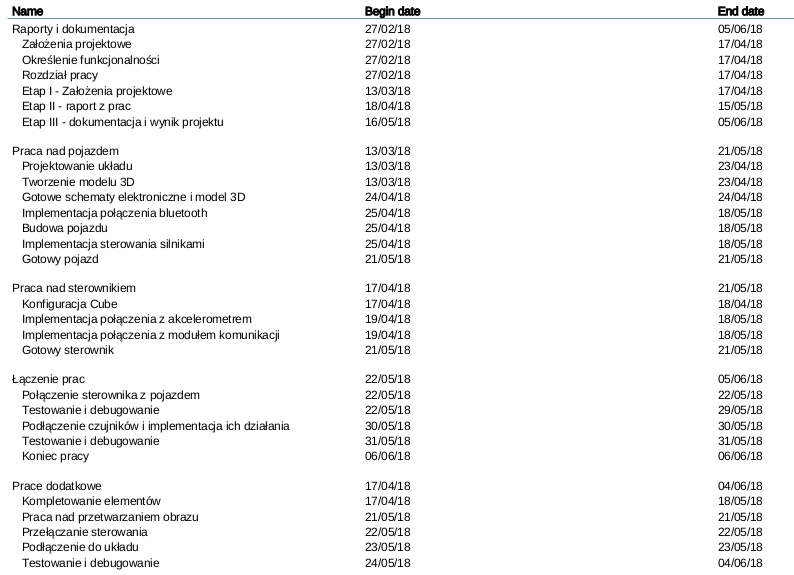
\includegraphics[width=0.8\textwidth]{Harm.png}
	\caption{Harmonogram pracy}
	\label{fig:Harmonogram}
\end{figure}


\newpage
\subsection{Podział pracy}
Podział pracy pomiędzy członków grupy został przedstawiony w tabeli \ref{tab:Tabela rozkladu pracy}.

\begin{table}[H]
	\centering
	\begin{tabular}{|p{7.8cm}|p{7.8cm}|} \hline
%	\begin{tabular}{|l|l|}

		\textbf{Patrycjusz } & \textbf{Maciej} \\ \hline \hline
		dobór elementów potrzebnych do realizacji projektu & konfiguracja Cube \\ \hline
		projekt 3D pojazdu & algorytm sterowania pojazdem za pomocą akcelerometru na płytce Discovery \\ \hline
		wydrukowanie modelu na drukarce 3D & testy poprawności działania algorytmu podłączając pojazd do płytki za pomocą kabla \\ \hline
		projekt elektroniki i płytki PCB &  algorytm sterowania pojazdem w momencie gdy zostanie wykryta przeszkoda  \\ \hline
		polutowanie układu oraz testy poprawności działania &  testy poprawności działania algorytmu podłączając pojazd do płytki za pomocą kabla \\ \hline
		podłączenie elektroniki i montaż elementów mechanicznych &--------------- \\ \hline
		\multicolumn{2}{|c|}{rozwój modułu komunikacji} \\ \hline
		\multicolumn{2}{|c|}{testy poprawności działania robota} \\ \hline
	\end{tabular}
	\caption{Tabela rozkładu zadań}	
	\label{tab:Tabela rozkladu pracy}
\end{table}

\noindent Biorąc pod uwagę przedstawiony rozkład pracy oraz jej harmonogram uwzględniający terminy oddania raportów z poszczególnych etapów projektu przystąpiono do stworzenia diagramu Gantta niniejszego projektu.

\newpage
\begin{landscape}
\subsection{Diagram Gantta}
Na podstawie stworzonego harmonogramu oraz rozkładu pracy wygenerowano diagram Gantta korzystając z programu Ganttproject.
Diagram przedstawiono na rysunku \ref{fig:Gantt}.


\begin{figure}[H]
	\centering
	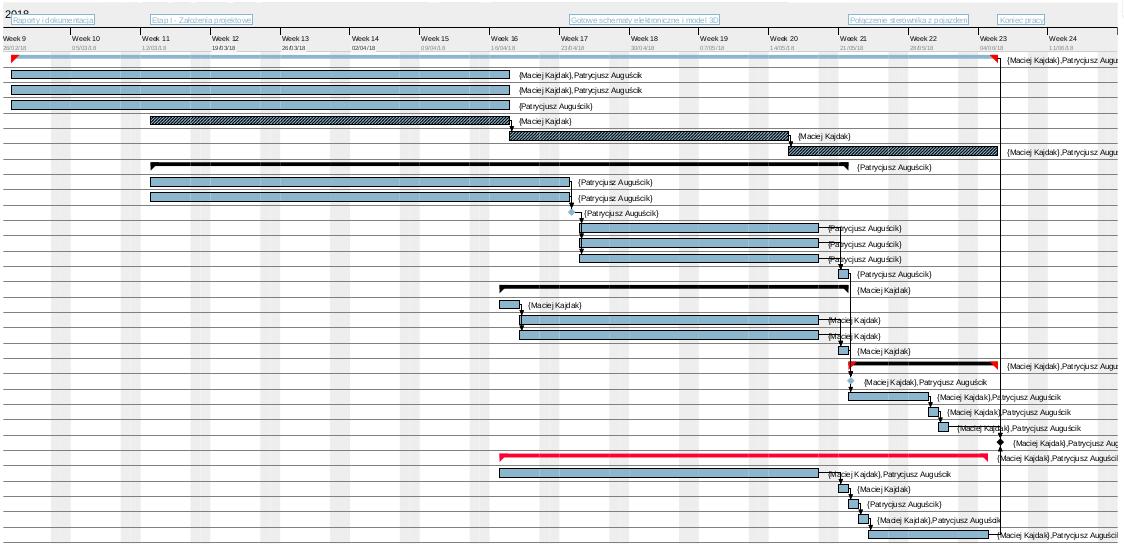
\includegraphics[scale=0.6, keepaspectratio]{GanttSR.png}
	\caption{Diagram Gantta}
	\label{fig:Gantt}
\end{figure}
\end{landscape}
%\newpage
%\section{Podsumowanie}


%\newpage
%	\section{Schematy elektroniczne}
%	\begin{figure}[H]
%		\centering	
%		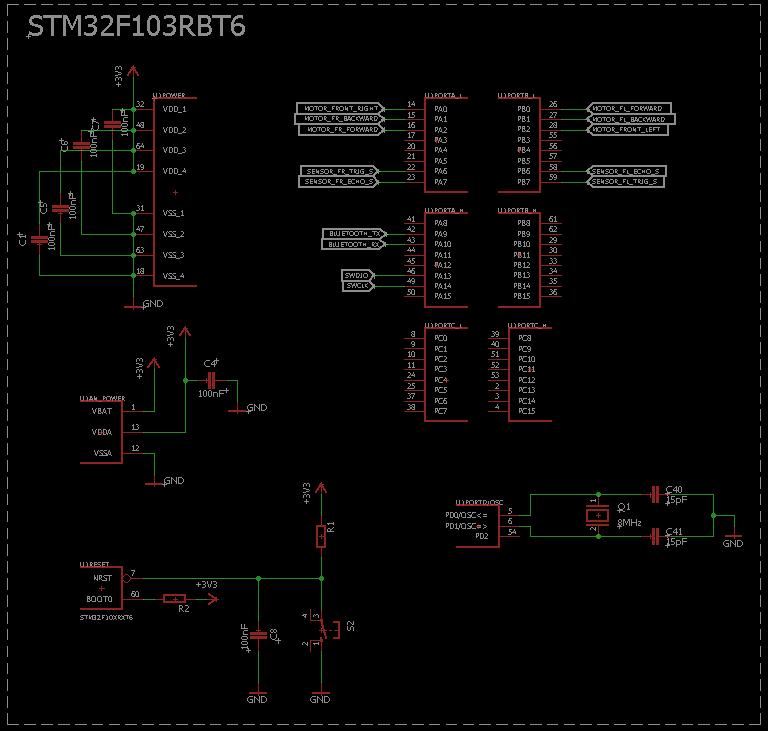
\includegraphics[scale=0.5, width=\textwidth ,height=\textheight ,keepaspectratio]{STM32.png}
%		\caption{Schemat polaczen STM32F103RBT6}
%	\end{figure}
%
%\begin{figure}[H]
%	\centering
%	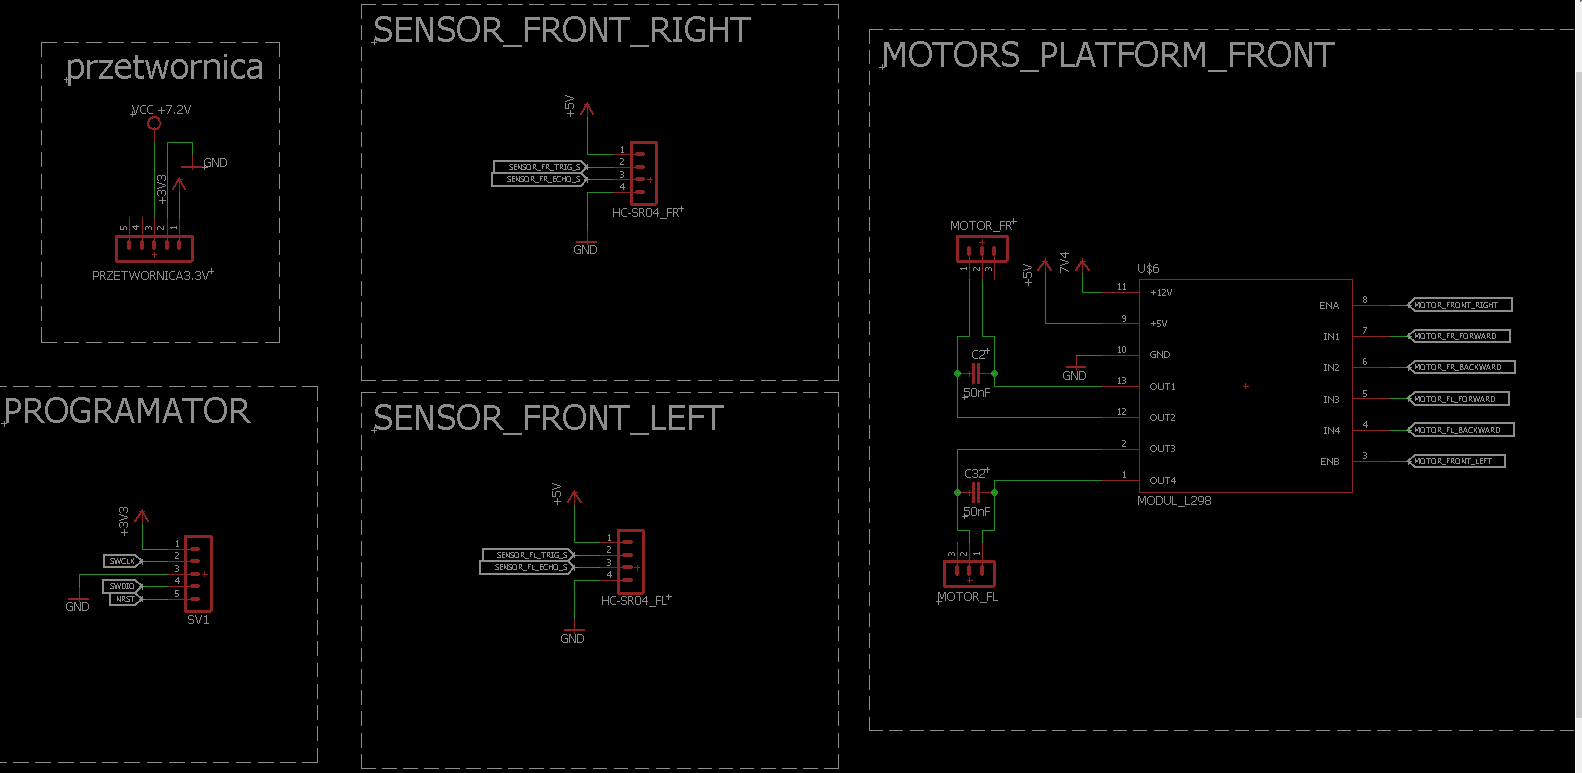
\includegraphics[scale=0.5, width=\textwidth ,height=\textheight ,keepaspectratio]{czujniki.png}
%	\caption{Schemat połączeń programatora, czujników odległości oraz mostka H}
%\end{figure}


%\addcontentsline{toc}{section}{Bibilografia}
%\bibliography{bibliografia}
%\bibliographystyle{plain}


\newpage
\listoffigures
\newpage
\listoftables


\end{document}







































